%
% The first command in your LaTeX source must be the \documentclass command.
\documentclass[sigconf]{acmart}

%
% \BibTeX command to typeset BibTeX logo in the docs
\AtBeginDocument{%
  \providecommand\BibTeX{{%
    \normalfont B\kern-0.5em{\scshape i\kern-0.25em b}\kern-0.8em\TeX}}}

\usepackage{multirow}
% Rights management information. 
% This information is sent to you when you complete the rights form.
% These commands have SAMPLE values in them; it is your responsibility as an author to replace
% the commands and values with those provided to you when you complete the rights form.
%
% These commands are for a PROCEEDINGS abstract or paper.
\copyrightyear{2019} 
\acmYear{2019} 
\setcopyright{acmlicensed}
\acmConference[WebSci '19]{11th ACM Conference on Web Science}{June 30-July 3, 2019}{Boston, MA, USA}
\acmBooktitle{11th ACM Conference on Web Science (WebSci '19), June 30-July 3, 2019, Boston, MA, USA}
\acmPrice{15.00}
\acmDOI{10.1145/3292522.3326046}
\acmISBN{978-1-4503-6202-3/19/06}

%
% These commands are for a JOURNAL article.
%\setcopyright{acmcopyright}
%\acmJournal{TOG}
%\acmYear{2018}\acmVolume{37}\acmNumber{4}\acmArticle{111}\acmMonth{8}
%\acmDOI{10.1145/1122445.1122456}

%
% Submission ID. 
% Use this when submitting an article to a sponsored event. You'll receive a unique submission ID from the organizers
% of the event, and this ID should be used as the parameter to this command.
%\acmSubmissionID{123-A56-BU3}

%
% The majority of ACM publications use numbered citations and references. If you are preparing content for an event
% sponsored by ACM SIGGRAPH, you must use the "author year" style of citations and references. Uncommenting
% the next command will enable that style.
%\citestyle{acmauthoryear}
\usepackage{verbatim}
%
% end of the preamble, start of the body of the document source.
\begin{document}

\begin{comment}

setwd(paste0(githubdir, "pwned_dev/ms/"))
tools::texi2dvi("pwned.tex", pdf = TRUE, clean = TRUE)
setwd(githubdir)

\end{comment}
%
% The "title" command has an optional parameter, allowing the author to define a "short title" to be used in page headers.
\title[Pwned]{Pwned: The Risk of Exposure in Data Breaches and its Predictors}

%
% The "author" command and its associated commands are used to define the authors and their affiliations.
% Of note is the shared affiliation of the first two authors, and the "authornote" and "authornotemark" commands
% used to denote shared contribution to the research.
\author{Gaurav Sood}
\authornotemark[1]
\email{gsood07@gmail.com}
\affiliation{%	\affiliation{%
  \institution{}
}

\author{Ken Cor}
\authornotemark[2]
\email{mcor@ualberta.ca}
\affiliation{%	\affiliation{%
  \institution{The University of Alberta}
  \city{Edmonton}
  \country{Canada}
}
%
% By default, the full list of authors will be used in the page headers. Often, this list is too long, and will overlap
% other information printed in the page headers. This command allows the author to define a more concise list
% of authors' names for this purpose.
\renewcommand{\shortauthors}{Sood and Cor}

%
% The abstract is a short summary of the work to be presented in the article.
\begin{abstract}
News about massive data breaches is increasingly common. But we do not know what proportion of Americans are exposed in these breaches. We combine data from a large, representative sample of American adults (n = 5,000), recruited by YouGov, with data from \textit{Have I Been Pwned} to estimate the lower bound of the number of times an average American's private information has been exposed. We find that at least 82.84\% of Americans have had their private information, including account credentials, Social Security Number, etc., exposed. On average, Americans' private information has been exposed in at least three breaches. The better educated, the middle-aged, women, and Whites are more likely to have had their accounts breached than the complementary groups.
\end{abstract}

%
% The code below is generated by the tool at http://dl.acm.org/ccs.cfm.
% Please copy and paste the code instead of the example below.
%
\begin{CCSXML}
<ccs2012>
<concept>
<concept_id>10002978.10003029.10003032</concept_id>
<concept_desc>Security and privacy~Social aspects of security and privacy</concept_desc>
<concept_significance>500</concept_significance>
</concept>
</ccs2012>
\end{CCSXML}

\ccsdesc[500]{Security and privacy~Social aspects of security and privacy}


%
% Keywords. The author(s) should pick words that accurately describe the work being
% presented. Separate the keywords with commas.
\keywords{Security risk, Privacy risk, Data breaches, Digital divide}

%
% A "teaser" image appears between the author and affiliation information and the body 
% of the document, and typically spans the page. 
%\begin{teaserfigure}
%  \includegraphics[width=\textwidth]{sampleteaser}
%  \caption{Seattle Mariners at Spring Training, 2010.}
%  \Description{Enjoying the baseball game from the third-base seats. Ichiro Suzuki preparing to bat.}
%  \label{fig:teaser}
%\end{teaserfigure}

%
% This command processes the author and affiliation and title information and builds
% the first part of the formatted document.
\maketitle

\section{Introduction}
On the Internet, nobody knows you're a dog. So the adage goes. But increasingly, others know that you like dog food and hate cats. Many of us have made our peace with this new reality. A slew of massive account breaches in recent years, however, threatens to pull the rug from under all illusions of anonymity \cite{mccandless}.\footnote{On September 22, 2016, for instance, Yahoo! revealed that 500M accounts had been compromised in a breach \cite{fiegerman}. Less than three months later, on December 14, 2016, Yahoo! announced that data had been stolen from nearly 1B user accounts in a different breach \cite{newman}. In all, Wikipedia lists 272 separate breaches between 2004 and 2018 (see \href{https://en.wikipedia.org/wiki/List_of_data_breaches}{https://en.wikipedia.org/wiki/List\_of\_data\_breaches})}

But there is little existing research on how frequently Americans' private information is part of such breaches. Much of the research on data breaches has focused on the downstream impact on corporations, e.g., \cite{whitler2017impact, rosati2019social, janakiraman2018effect}, and people, e.g., \cite{cross2019media, mikhed2018data, curtis2018consumer}. Such research is vital---it informs data breach notification policy and laws, e.g., \cite{nieuwesteeg2018analysis, marcus2018data, kuhn2018147}. But absent from the literature is data that is important for developing effective public policy and laws on corporate liability for data breaches---data on the average American's risk of their private information being exposed in a data breach. In this note, we shed light on this mostly unexplored question. 

Using a unique dataset, we estimate the lower bound of the average number of breached online accounts per person. We merge data from a large representative sample from YouGov (n = 5,000) with data from \href{https://haveibeenpwned.com}{Have I Been Pwned} (HIBP). We check whether the email associated with the YouGov account is part of the 293 public breaches cataloged by HIBP. We also study how exposure to breaches varies by socio-economic factors including ethnicity, sex, age, and education.

\section{Data and Methods}
In July 2018, YouGov drew a nationally representative sample of 5,000 adult Americans. YouGov draws the sample as follows: it starts with a random sample of a high-quality sample of American adults, e.g., Current Population Survey, and then finds people on its panel that match the drawn sample most closely \cite{rivers}. Some research suggests that the quality of samples drawn by YouGov is comparable to those drawn using probability sampling \cite{ansolabehere}. The sample that YouGov drew here, however, is better than its traditional survey samples. Non-response bias in our sample is zero because YouGov did not have to send out surveys; it used the emails associated with the accounts to collect the data. (YouGov never shared the emails with us.) Table~\ref{table:yg_dat} presents the marginals on key socio-demographic variables (see \href{https://github.com/themains/pwned/tree/master/data}{here} for the codebook). (Table~\ref{table:cps_yg} presents the comparison between the Current Population Survey (CPS) and YouGov on key demographic variables. The upshot is that on key marginals, the difference between YouGov and CPS is less than 5\%.)

\begin{table}[h!]
\centering
\caption{YouGov Sample Characteristics}
\begin{tabular}{ l c }
\hline    
 & proportion \\
\hline
race   & \\
\hspace{2mm}white            &  .67\\
\hspace{2mm}hispanic/latino  &  .13\\
\hspace{2mm}black            &  .12\\
\hspace{2mm}asian            &  .03\\
\hspace{2mm}middle eastern   &  .02\\
\hspace{2mm}mixed race       &  .01\\
\hspace{2mm}native american  &  .01\\
\hspace{2mm}other            &  .00\\
& \\
sex & \\
\hspace{2mm}female           &  .54\\
& \\
age & \\
\hspace{2mm}(18, 25]     & .09 \\
\hspace{2mm}(25, 35]     & .19 \\
\hspace{2mm}(35, 50]     & .26 \\
\hspace{2mm}(50, 65]     & .28 \\
\hspace{2mm}(65, 100]    & .18 \\
& \\
education & \\
\hspace{2mm}no hs                 &   .06\\
\hspace{2mm}hs grad.            &     .32\\
\hspace{2mm}some college        &     .20\\
\hspace{2mm}2-year college degree &   .11\\
\hspace{2mm}4-year college degree &   .19\\
\hspace{2mm}postgrad degree       &   .11\\
\hline
\end{tabular}
\label{table:yg_dat}
\end{table}

After drawing the sample, YouGov used the emails associated with the accounts to query the HIBP API. (YouGov did the lookups so that it didn't have to share the email IDs.) HIBP is a non-profit clearinghouse of information about online account breaches. HIBP's stated aim is to provide a way for people to check if they are at risk from online breaches. It currently carries data from 293 breaches covering 278 unique domains and 5,235,843,322 accounts, including data from prominent breaches like the two Yahoo! breaches covering nearly 1.5 billion accounts. The HIPB data are, however, not comprehensive. Security researchers believe that there are many breaches that the companies are unaware of and at least a few cases where a company doesn't share information about a breach it knows about. HIBP also refuses to provide data on sensitive breaches---breached accounts where a person's inclusion may adversely affect them---from their public API\footnote{HIBP website notes that it does not share whether or not an account has been part of the breach at Adult Friend Finder, Ashley Madison, Beautiful People, Bestialitysextaboo, Brazzers, CrimeAgency vBulletin Hacks, Fling, Florida Virtual School, Freedom Hosting II, Fridae, Fur Affinity, HongFire, Mate1.com, Muslim Match, Naughty America, Non Nude Girls, Rosebutt Board, The Candid Board, The Fappening, xHamster and 1 more.}.  So data from HIBP only gives us a lower bound.

HIPB provides an easy way to get all the breached accounts associated with a particular email ID---you just need to make a simple API call passing the email that you want to get data on. This method gives us data on all the breaches logged by HIPB for all the 5,000 profiles. There is one caveat.  Our YouGov sample provides data associated with only one email ID, the email people used to register with YouGov. People often have multiple email IDs. And that is another reason why all we get from this data is a lower bound. The actual number of breached accounts per person is likely much higher. 

With each request, HIBP returns some metadata on the kind of breaches. (See the \href{https://github.com/themains/pwned/blob/master/data/Profile_codebook_ygov1058.pdf}{codebook} for details about all the data that it returns.) Two pieces of information are material here. HIBP classifies each breach as verified or unverified. And it defines unverified breaches as breaches whose ``legitimacy'' it cannot ``establish beyond [a] reasonable doubt.'' HIBP includes these unverified breaches because ``they still contain personal information about individuals who want to understand their exposure on the web.'' The other material column that HIBP returns relates to whether a breach is part of a ``spam list.'' HIBP defines {\it SpamList} as cases where ``large volumes of personal data are found being utilized for the purposes of sending targeted spam.'' HIBP adds, ``This often includes many of the same attributes frequently found in data breaches such as names, addresses, phones numbers and dates of birth. The lists are often aggregated from multiple sources, frequently by eliciting personal information from people with the promise of a monetary reward.'' And the reason HIBP includes these data is: ``whilst the data may not have been sourced from a breached system, the personal nature of the information and the fact that it's redistributed in this fashion unbeknownst to the owners warrants inclusion here.''

\section{Results}

In all, 14,979 breaches are associated with the 5,000 emails on file. Or on average, there are three breaches per person. The median is also three. And at least 82.84\% of Americans' accounts have been breached at least once. 

The relationship between the number of breaches and socio-economic is counter to what focusing on traditional concerns around the digital divide would lead us to believe. If anything, the data suggest that people who use online services more are somewhat more likely to have their accounts breached. (See \ref{fig:si_tables} and \ref{fig:si_figs} for corresponding regressions and figures illustrating group-wise means along with the 95\% confidence intervals.) 

The number of breaches increases roughly monotonically with education (see Table~\ref{tab:educ_breaches} and Figure~\ref{fig:educ_breaches}). The average number of breaches among people with no high school degree is 2.35. Compare this to postgraduates, who are part of 3.20 breaches on average (or 1.3 times the average of people with no high school degree).

In contrast to the relationship between education and the number of breaches, the relationship between the number of breaches and age is curvilinear (see Table \ref{tab:age_breaches}), with young people's and seniors' accounts least likely to be breached, and middle-aged adults' accounts most likely to be breached. But, as the loess illustrates (see Figure \ref{fig:age_breaches}), the relationship is modest.

% latex table generated in R 3.5.3 by xtable 1.8-4 package
% Sat Apr 27 17:55:55 2019
\begin{table}[!htb]
\centering
\caption{Frequency of Account Breaches By Socio-economic Factors} 
\label{table:socdem_dat}
\begingroup\small
\begin{tabular}{lrr}
  \hline
 & mean & se \\ 
  \hline
Age &  &  \\ 
  (18,25] & 1.96 & 0.10 \\ 
  (25,35] & 3.12 & 0.09 \\ 
  (35,50] & 3.34 & 0.08 \\ 
  (50,65] & 3.29 & 0.07 \\ 
  (65,100] & 2.95 & 0.07 \\ 
  Missing & 1.19 & 0.16 \\ 
   &  &  \\ 
  Education &  &  \\ 
  No HS & 2.35 & 0.12 \\ 
  HS Grad. & 2.89 & 0.06 \\ 
  Some College & 3.04 & 0.09 \\ 
  2-year College Degree & 3.07 & 0.10 \\ 
  4-year College Degree & 3.22 & 0.09 \\ 
  Postgrad Degree & 3.20 & 0.11 \\ 
   &  &  \\ 
  Sex &  &  \\ 
  Female & 3.17 & 0.05 \\ 
  Male & 2.82 & 0.05 \\ 
   &  &  \\ 
  Race &  &  \\ 
  White & 3.12 & 0.05 \\ 
  Black & 3.16 & 0.11 \\ 
  Hispanic/Latino & 2.50 & 0.08 \\ 
  Asian & 2.82 & 0.21 \\ 
  Native American & 2.96 & 0.26 \\ 
  Middle Eastern & 2.66 & 0.24 \\ 
  Mixed Race & 2.45 & 0.22 \\ 
  Other & 2.92 & 1.32 \\ 
   \hline
\end{tabular}
\endgroup
\end{table}


When we compare the average number of breaches among men and women, we find that women's accounts are 1.12 times more likely to be breached than men's (see Table ~\ref{table:socdem_dat} and \ref{tab:sex_breaches}; $p < .05$). Analyzing breaches by ethnicity, Blacks' and Whites' accounts are most frequently breached. The mean number of breaches associated with the emails for Blacks and Whites is 3.12 and 3.16 respectively. For Hispanics/Latinos, the corresponding number is 2.5 (see Table \ref{tab:race_breaches}; $p < .05$). And for Asians, the mean is 2.82.

To assess the source of the exposure, we checked the source of the breaches. The 14,979 breaches stemmed from 156 different sites, but there was a sharp skew with 21 sites with more than 100 breaches accounting for 11,783 of the breaches. Table ~\ref{table:domain_dat} lists the 21 sites. Prominent websites like \url{linkedin.com}, \url{adobe.com}, \url{dropbox.com}, \url{lastfm.com}, among others feature on the list.

\begin{table}[h!]
\centering
\caption{Most Frequently Implicated Domains}
\begin{tabular}{ l c }
\hline    
domain name & n \\
\hline
rivercitymediaonline.com &   2,913 \\
linkedin.com             &   1,089 \\
modbsolutions.com        &   1,067\\
myspace.com              &   1,059\\
data4marketers.com       &    996\\
cashcrate.com            &    856\\
adobe.com                &    609\\
disqus.com               &    570\\
ticketfly.com            &    393\\
tumblr.com               &    340\\
dropbox.com              &    288\\
dailymotion.com          &    255\\
last.fm                  &    248\\
evony.com                &    171\\
clixsense.com            &    150\\
cafemom.com              &    145\\
imesh.com                &    144\\
kickstarter.com          &    140\\
edmodo.com               &    130\\
zomato.com               &    112\\
neopets.com              &    108\\
\hline
\end{tabular}
\label{table:domain_dat}
\end{table}

In the analysis presented until now, we don't distinguish between different kinds of breaches. But not all breaches are equally grave. So next, we shed light on the type of breaches.  Of the 15,837 breaches, 14,979 or 94.58\% were part of verified breaches. And about a third of the 15,837 breaches are categorized as {\it SpamList}. In all, we have 10,188 breaches that are verified and not categorized as {\it SpamList}. We focus our attention on these plausibly graver breaches, checking whether the relationship with socio-economic variables we see above hold in this smaller subset. 

% latex table generated in R 3.5.3 by xtable 1.8-4 package
% Sat Apr 27 17:56:00 2019
\begin{table}[!htb]
\centering
\caption{Frequency of Verified, Non-SpamList Account Breaches By Socioeconomic Factors.} 
\label{table:socdem_verified_dat}
\begingroup\small
\begin{tabular}{lrr}
  \hline
 & mean & se \\ 
  \hline
Age &  &  \\ 
  (18,25] & 1.63 & 0.10 \\ 
  (25,35] & 2.44 & 0.08 \\ 
  (35,50] & 2.37 & 0.07 \\ 
  (50,65] & 2.16 & 0.06 \\ 
  (65,100] & 1.78 & 0.05 \\ 
  Missing & 0.91 & 0.13 \\ 
   &  &  \\ 
  Education &  &  \\ 
  No HS & 1.53 & 0.09 \\ 
  HS Grad. & 1.91 & 0.05 \\ 
  Some College & 2.22 & 0.08 \\ 
  2-year College Degree & 2.10 & 0.08 \\ 
  4-year College Degree & 2.37 & 0.08 \\ 
  Postgrad Degree & 2.30 & 0.08 \\ 
   &  &  \\ 
  Sex &  &  \\ 
  Female & 2.15 & 0.04 \\ 
  Male & 2.05 & 0.05 \\ 
   &  &  \\ 
  Race &  &  \\ 
  White & 2.21 & 0.04 \\ 
  Black & 2.03 & 0.08 \\ 
  Hispanic/Latino & 1.73 & 0.07 \\ 
  Asian & 2.16 & 0.18 \\ 
  Native American & 1.85 & 0.18 \\ 
  Middle Eastern & 2.05 & 0.21 \\ 
  Mixed Race & 1.70 & 0.19 \\ 
  Other & 2.69 & 1.19 \\ 
   \hline
\end{tabular}
\endgroup
\end{table}


When we look at education, the pattern holds up. Once again, the number of breached accounts per person for people with a college degree or more is higher than for people who only got as far as high school (see Table \ref{table:socdem_verified_dat}). Moving to sex, the pattern is more attenuated with women just nudging ahead of men---the mean for women and men is 2.15 and 2.05 respectively.  The general pattern for age remains roughly similar to what we saw above, with the middle-aged more likely to have their accounts breached compared to people younger than 25 and older than 65. Breaking down by race, we see some interesting changes. Asians join Whites near the top of the pile, with means of about 2.2. Accounts of Hispanics or Latinos are less likely to be part of verified non-spam-list breaches (mean = 1.73, $p < .05$). The big relative change is for Blacks; African-Americans are likelier to be part of unverified, {\it SpamList} breaches.

\section{Conclusion}

Nearly 83\% of Americans' have had their accounts breached at least once. In total, the 5,000 email accounts on file are associated with 14,979 breaches. Or, on average, people's accounts have been breached thrice. This number, though, is the lower bound for three reasons. First, not all breaches are made public. Second, HIBP doesn't allow access to data on sensitive breaches---breached online accounts on services that may have reputational consequences for people---via its public API. Third, many Americans have multiple email accounts. We only had one email ID per person. 

We also find that the kinds of people who are most likely to use online services---the better educated, Whites, etc.---are generally the most exposed. This finding is consistent with Laohaprapanon and Sood, who find that the better educated, people with higher incomes, and racial majorities spend a smaller proportion of time online on problematic sites, but because they are online more often, they end up visiting more such sites \cite{laohaprapanon}. This is contrary to the traditional narrative about the digital divide \cite{van2011internet}.

\clearpage
\bibliographystyle{ACM-Reference-Format}
\bibliography{pwned}

\clearpage
\appendix
\renewcommand{\thesection}{SI \arabic{section}}
\setcounter{table}{0}\renewcommand\thetable{\thesection.\arabic{table}}  
\setcounter{figure}{0}\renewcommand\thefigure{\thesection.\arabic{figure}}
\counterwithin{figure}{section}

\section{Supporting Information}

\subsection{Tables}
\label{fig:si_tables}

The missing entries reflect cases where we do not have commensurate categories in our data. The largest differences we see are on race and ethnicity, a variable where our coding differs from CPS in meaningful ways. 

% latex table generated in R 3.5.3 by xtable 1.8-4 package
% Mon Apr 29 20:09:37 2019
\begin{table}[!htb]
\centering
\caption{Comparison Between YouGov and CPS 2018} 
\label{table:cps_yg}
\begingroup\small
\begin{tabular}{lrrr}
  \hline
 & cps & yg & diff \\ 
  \hline
Age &  &  &  \\ 
  18 to 25 & 0.14 & 0.13 & 0.01 \\ 
  26 to 35 & 0.18 & 0.18 & 0.00 \\ 
  36 to 50 & 0.25 & 0.23 & 0.02 \\ 
  51 to 65 & 0.25 & 0.26 & -0.01 \\ 
  66 to 80+ & 0.19 & 0.18 & 0.01 \\ 
  Sex &  &  &  \\ 
  Male & 0.48 & 0.51 & -0.03 \\ 
  Female & 0.52 & 0.49 & 0.03 \\ 
  Race &  &  &  \\ 
  White alone & 0.78 & 0.64 & 0.14 \\ 
  Black or African American alone & 0.13 & 0.12 & 0.01 \\ 
  American Indian and Alaska Native alone & 0.01 & 0.01 & 0.00 \\ 
  Asian alone & 0.06 &  &  \\ 
  Native Hawaiian and Other Pacific Islander alone & 0.00 &  &  \\ 
  Two or more races & 0.02 &  &  \\ 
  Educational Attainment &  &  &  \\ 
  No high school diploma & 0.11 & 0.07 & 0.04 \\ 
  High school or equivalent & 0.29 & 0.33 & -0.04 \\ 
  Some college, less than 4-yr degree & 0.28 & 0.31 & -0.03 \\ 
  Bachelor's degree or higher & 0.32 & 0.29 & 0.03 \\ 
   \hline
\end{tabular}
\endgroup
\end{table}

\clearpage


% Table created by stargazer v.5.2.2 by Marek Hlavac, Harvard University. E-mail: hlavac at fas.harvard.edu
% Date and time: Sat, Apr 27, 2019 - 5:55:59 PM
\begin{table}[!htbp] \centering 
  \caption{Number of Breaches by Race/Ethnicity} 
  \label{tab:race_breaches} 
\begin{tabular}{@{\extracolsep{5pt}}lc} 
\\[-1.8ex]\hline 
\hline \\[-1.8ex] 
 & \multicolumn{1}{c}{\textit{Dependent variable:}} \\ 
\cline{2-2} 
\\[-1.8ex] & Number of Breaches \\ 
\hline \\[-1.8ex] 
 Black & .04 \\ 
  & (.12) \\ 
  Hispanic/Latino & $-$.62$^{***}$ \\ 
  & (.10) \\ 
  Asian & $-$.30 \\ 
  & (.23) \\ 
  Native American & $-$.16 \\ 
  & (.36) \\ 
  Middle Eastern & $-$.46$^{**}$ \\ 
  & (.24) \\ 
  Mixed Race & $-$.67$^{**}$ \\ 
  & (.29) \\ 
  Other & $-$.20 \\ 
  & (.73) \\ 
  Constant & 3.12$^{***}$ \\ 
  & (.05) \\ 
 \hline \\[-1.8ex] 
Observations & 5,000 \\ 
R$^{2}$ & .01 \\ 
Adjusted R$^{2}$ & .01 \\ 
\hline 
\hline \\[-1.8ex] 
\textit{Note:}  & \multicolumn{1}{r}{$^{*}$p$<$0.1; $^{**}$p$<$0.05; $^{***}$p$<$0.01} \\ 
\end{tabular} 
\end{table} 

\clearpage


% Table created by stargazer v.5.2.2 by Marek Hlavac, Harvard University. E-mail: hlavac at fas.harvard.edu
% Date and time: Sun, Feb 17, 2019 - 2:48:10 PM
\begin{table}[!htbp] \centering 
  \caption{Number of Breaches by Sex} 
  \label{} 
\begin{tabular}{@{\extracolsep{5pt}}lc} 
\\[-1.8ex]\hline 
\hline \\[-1.8ex] 
 & \multicolumn{1}{c}{\textit{Dependent variable:}} \\ 
\cline{2-2} 
\\[-1.8ex] & Number of Breaches \\ 
\hline \\[-1.8ex] 
 Male & $-$.35$^{***}$ \\ 
  & (.07) \\ 
  Constant & 3.17$^{***}$ \\ 
  & (.05) \\ 
 \hline \\[-1.8ex] 
Observations & 5,000 \\ 
R$^{2}$ & .004 \\ 
Adjusted R$^{2}$ & .004 \\ 
\hline 
\hline \\[-1.8ex] 
\textit{Note:}  & \multicolumn{1}{r}{$^{*}$p$<$0.1; $^{**}$p$<$0.05; $^{***}$p$<$0.01} \\ 
\end{tabular} 
\end{table} 

\clearpage


% Table created by stargazer v.5.2.2 by Marek Hlavac, Harvard University. E-mail: hlavac at fas.harvard.edu
% Date and time: Sat, Apr 27, 2019 - 5:55:59 PM
\begin{table}[!htbp] \centering 
  \caption{Number of Breaches by Education} 
  \label{tab:educ_breaches} 
\begin{tabular}{@{\extracolsep{5pt}}lc} 
\\[-1.8ex]\hline 
\hline \\[-1.8ex] 
 & \multicolumn{1}{c}{\textit{Dependent variable:}} \\ 
\cline{2-2} 
\\[-1.8ex] & Number of Breaches \\ 
\hline \\[-1.8ex] 
 HS Grad. & .54$^{***}$ \\ 
  & (.16) \\ 
  Some College & .69$^{***}$ \\ 
  & (.16) \\ 
  2-year College Degree & .72$^{***}$ \\ 
  & (.18) \\ 
  4-year College Degree & .87$^{***}$ \\ 
  & (.17) \\ 
  Postgrad Degree & .85$^{***}$ \\ 
  & (.18) \\ 
  Constant & 2.35$^{***}$ \\ 
  & (.14) \\ 
 \hline \\[-1.8ex] 
Observations & 5,000 \\ 
R$^{2}$ & .01 \\ 
Adjusted R$^{2}$ & .01 \\ 
\hline 
\hline \\[-1.8ex] 
\textit{Note:}  & \multicolumn{1}{r}{$^{*}$p$<$0.1; $^{**}$p$<$0.05; $^{***}$p$<$0.01} \\ 
\end{tabular} 
\end{table} 


\clearpage

% Table created by stargazer v.5.2.2 by Marek Hlavac, Harvard University. E-mail: hlavac at fas.harvard.edu
% Date and time: Mon, Feb 11, 2019 - 7:51:27 PM
\begin{table}[!htbp] \centering 
  \caption{Number of Breaches by Age} 
  \label{} 
\begin{tabular}{@{\extracolsep{5pt}}lc} 
\\[-1.8ex]\hline 
\hline \\[-1.8ex] 
 & \multicolumn{1}{c}{\textit{Dependent variable:}} \\ 
\cline{2-2} 
\\[-1.8ex] & Number of Breaches \\ 
\hline \\[-1.8ex] 
 ns(age, 2)1 & 2.23$^{***}$ \\ 
  & (.20) \\ 
  ns(age, 2)2 & $-$.90$^{***}$ \\ 
  & (.21) \\ 
  Constant & 2.01$^{***}$ \\ 
  & (.09) \\ 
 \hline \\[-1.8ex] 
Observations & 5,000 \\ 
R$^{2}$ & .03 \\ 
Adjusted R$^{2}$ & .03 \\ 
\hline 
\hline \\[-1.8ex] 
\textit{Note:}  & \multicolumn{1}{r}{$^{*}$p$<$0.1; $^{**}$p$<$0.05; $^{***}$p$<$0.01} \\ 
\end{tabular} 
\end{table} 


\clearpage
\subsection{Figures}
\label{fig:si_figs}

\begin{figure}[H]
  \centering
  \captionsetup{font={small,it}}
   \caption{Relationship Between Race and Number of Breaches
  \label{fig:race_breaches}}
    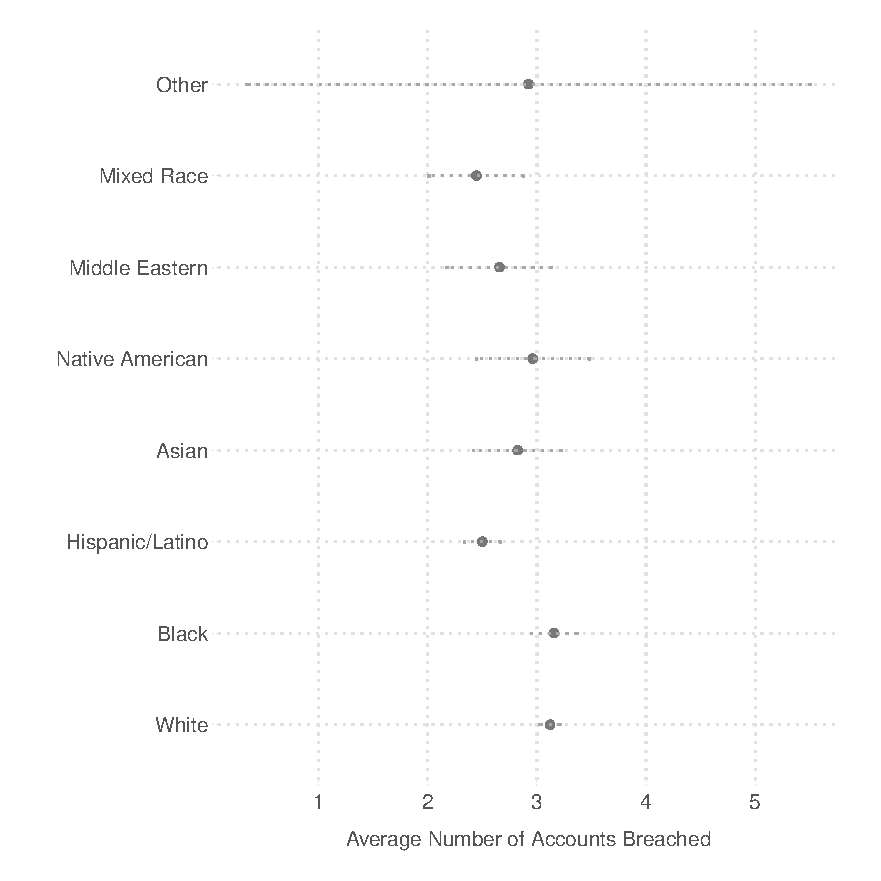
\includegraphics[scale=.75]{../figs/race_pwned.pdf}
\end{figure}
\clearpage

\begin{figure}[H]
  \centering
  \captionsetup{font={small,it}}
   \caption{Relationship Between Sex and Number of Breaches  
  \label{fig:sex_breaches}}
    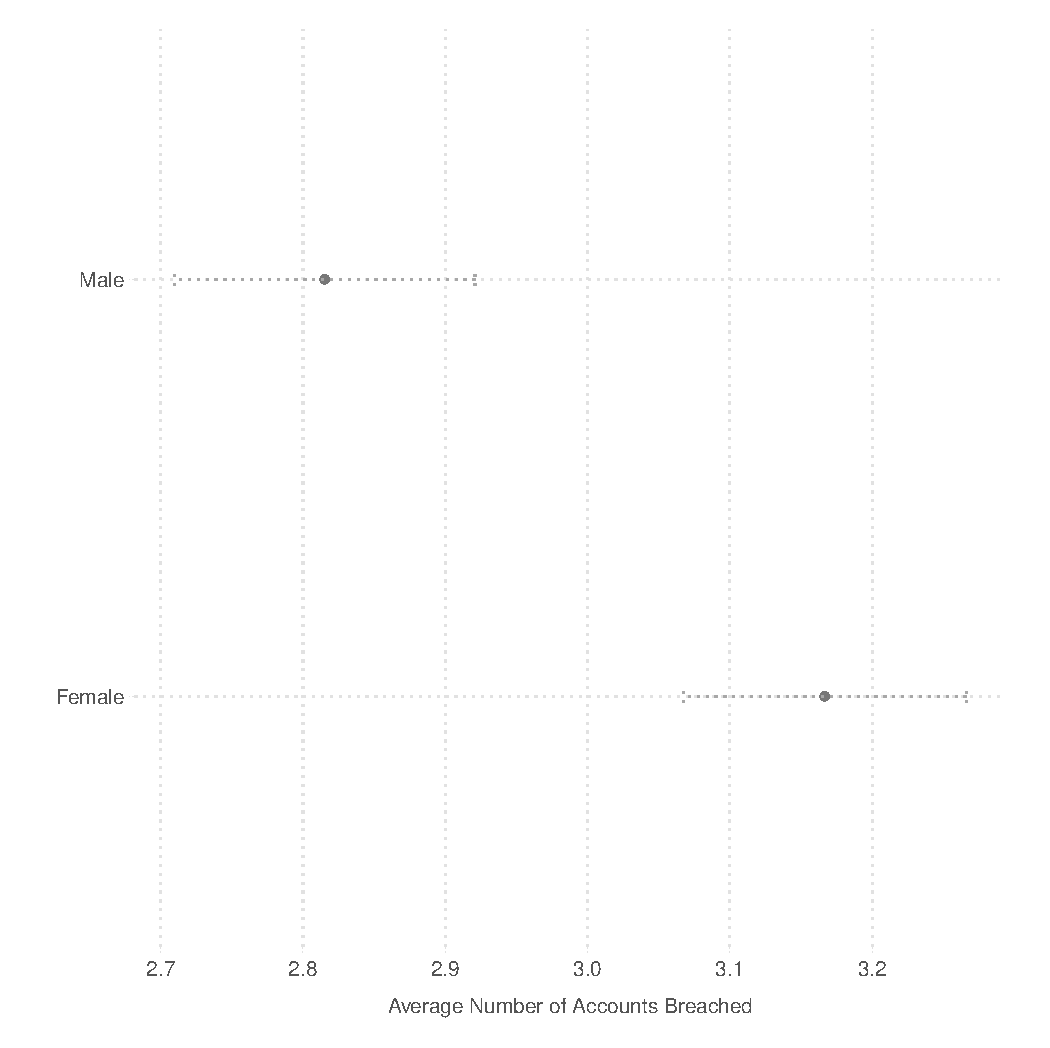
\includegraphics[scale=.75]{../figs/sex_pwned.pdf}
\end{figure}
\clearpage

\begin{figure}[H]
  \centering
  \captionsetup{font={small,it}}
   \caption{Relationship Between Education and Number of Breaches 
  \label{fig:educ_breaches}}
    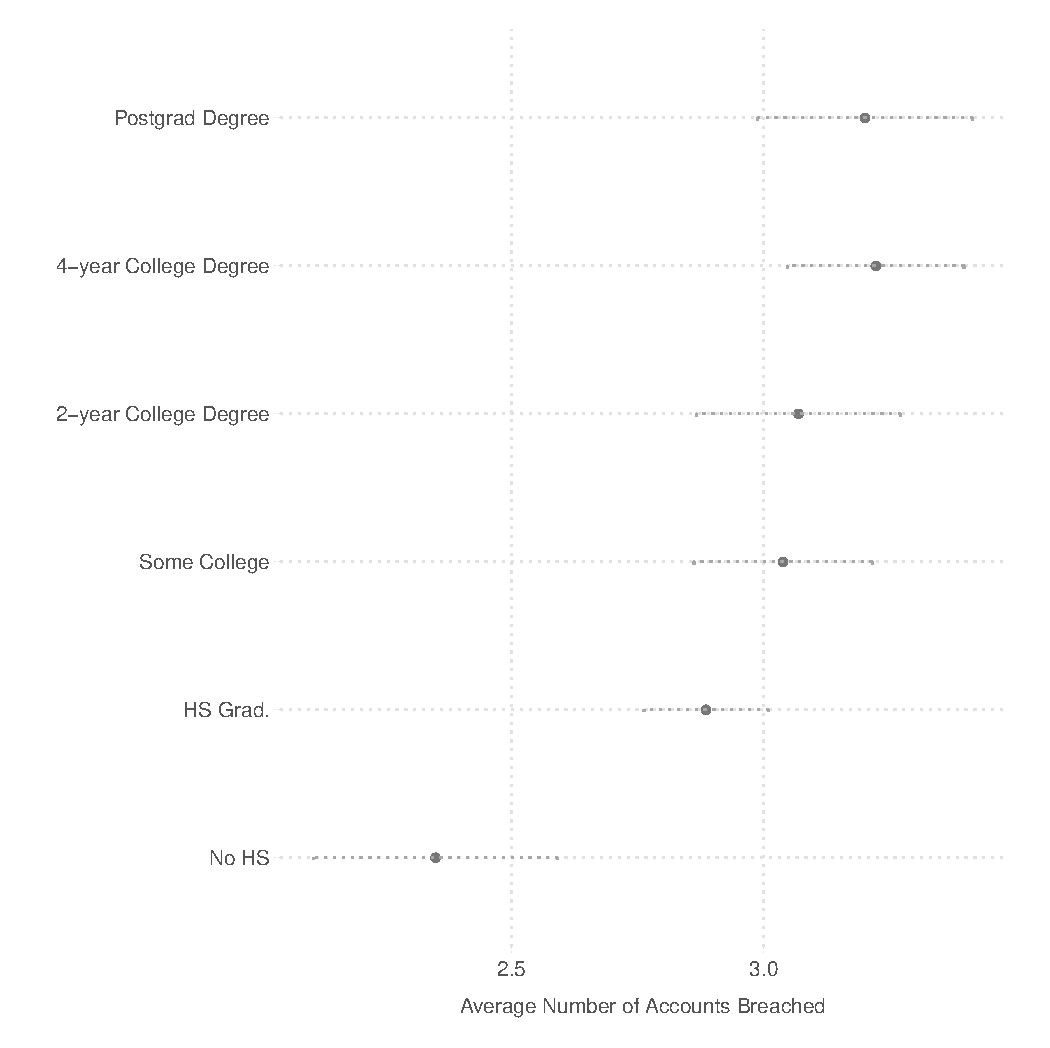
\includegraphics[scale=.75]{../figs/educ_pwned.pdf}
\end{figure}
\clearpage

\begin{figure}[H]
  \centering
  \captionsetup{font={small,it}}
   \caption{Relationship Between Age and Number of Breaches  
  \label{fig:age_breaches}}
    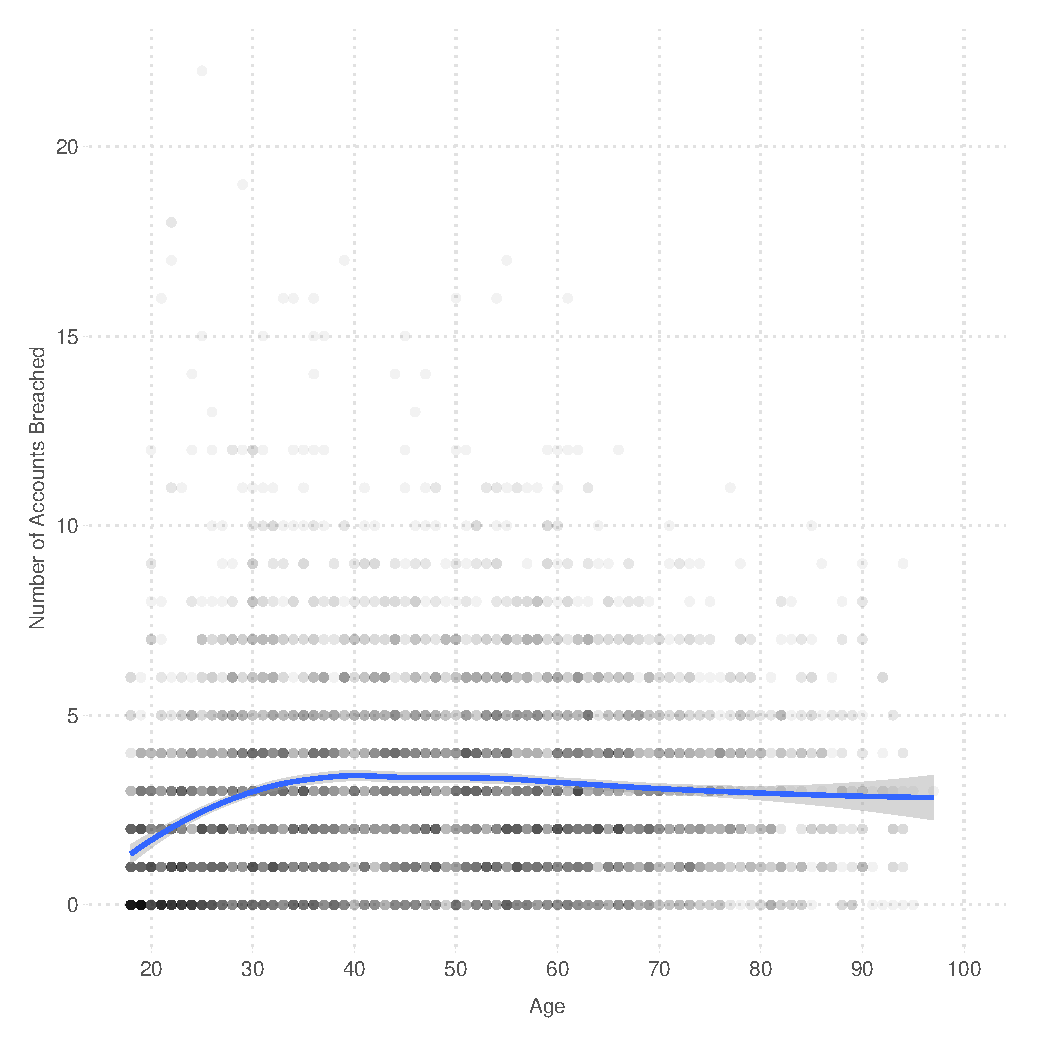
\includegraphics[scale=.75]{../figs/age_pwned.pdf}
\end{figure}

\end{document}